

\section{Ausgangssituation}
\label{sec: initial_situation}
\setauthor{David Altenhofer}
Seit Jahren müssen die Mitarbeiter der Firma die Datenbank
Einträge sehr umständlich ändern, da kein User Interface dafür 
vorhanden ist. Unser Ziel war es, genau das zu Ändern. Ich habe gemeinsam
mit meinem Team ein Web-Frontend erstellt, welches das Hinzufügen, Bearbeiten
und Löschen der Einträge in der Datenbank um ein vielfaches vereinfacht.
Nun kann auf das unpraktische Verwenden von Swagger verzichtet werden und auf ein paar 
wenige Klicks reduziert werden. 
\\
\\
Gegeben war bereits ein fertiges Backend mit einer API

\clearpage  

\begin{figure}[p]
    \centering
    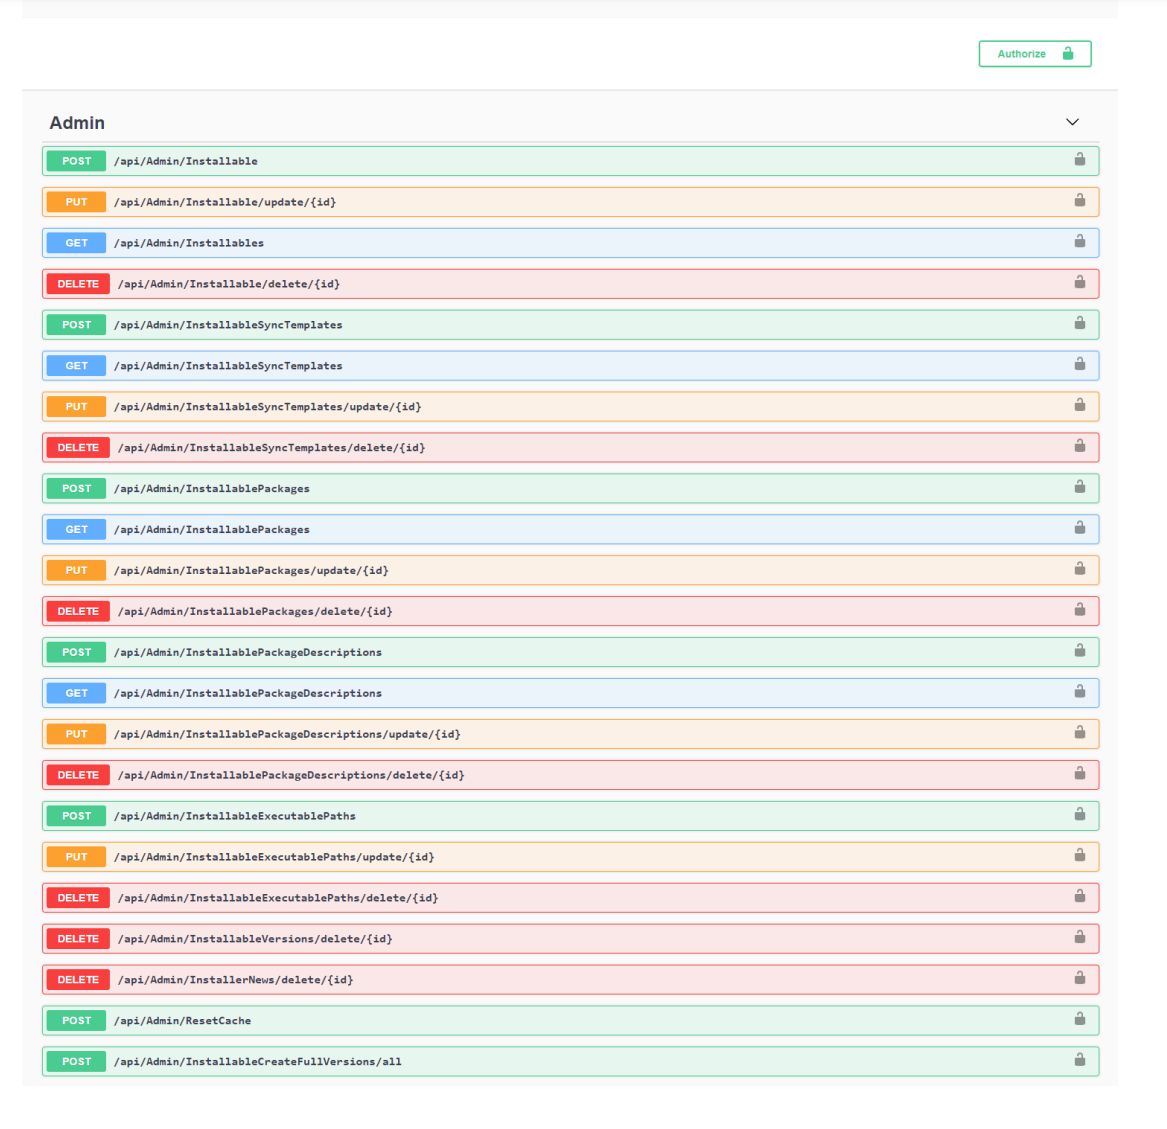
\includegraphics[width=.94\textwidth]{pics/swagger01.PNG}
    \caption{Swagger UI - Endpoints}
\end{figure}
\clearpage
\begin{figure}[p]
    \centering
    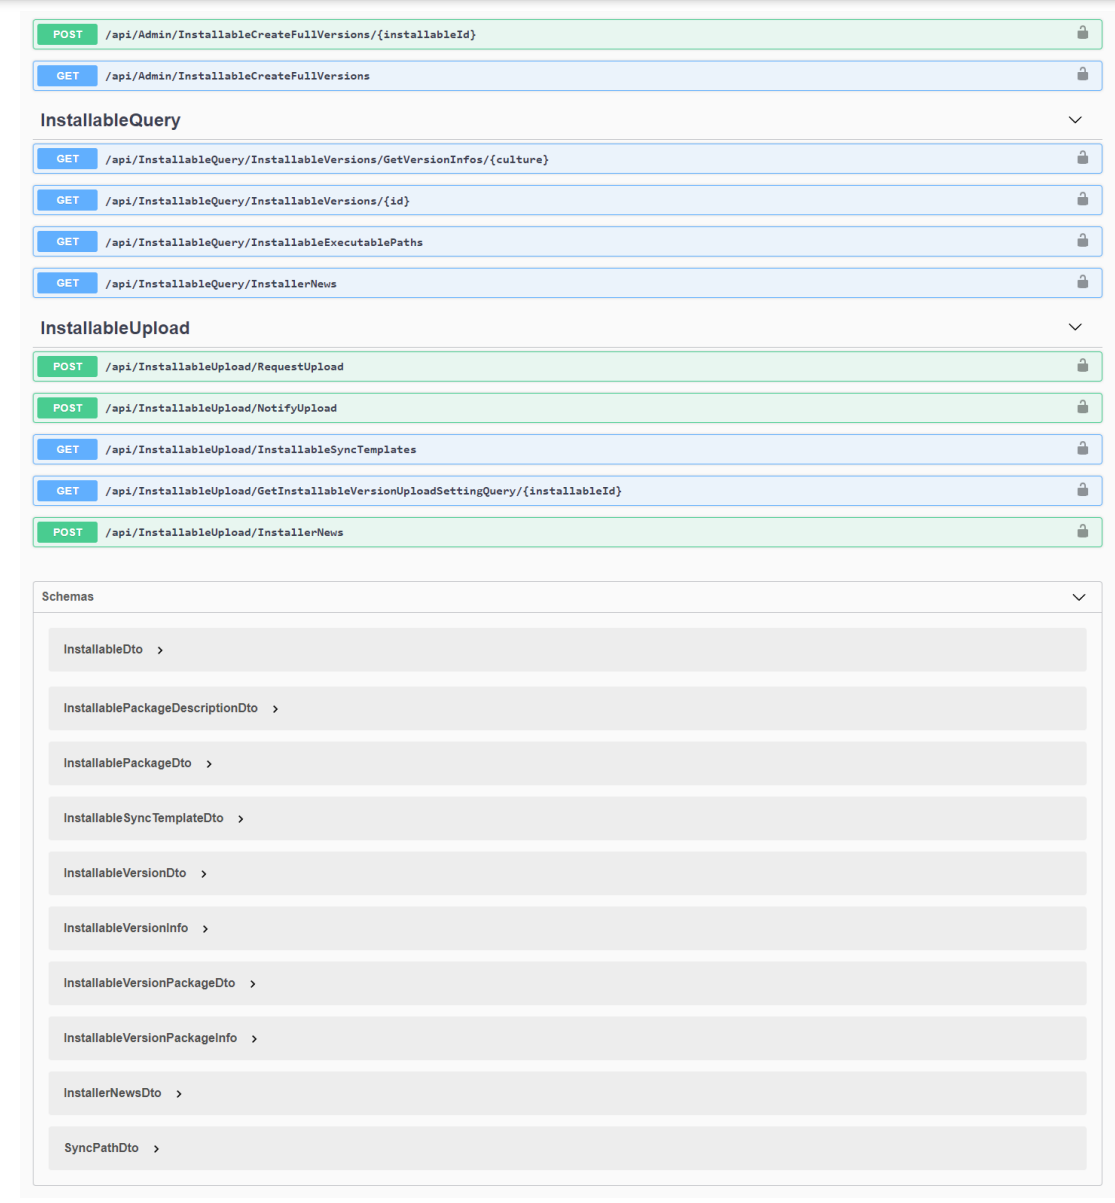
\includegraphics[width=.94\textwidth]{pics/swagger02.PNG}
    \caption{Swagger UI - Endpoints}
\end{figure}

\clearpage

\section{Aufgabenstellung}
\setauthor{David Altenhofer}
Um den Umgang mit der Datenbank für alle Mitarbeiter zu vereinfachen, soll ein leicht verständliches, inuitives Interface entwickelt werden.
Die Web-Anwendung darf nur für autorisierte Benutzer in der Abteilung der Firma verfügbar sein. Deswegen ist eine Authentifizierungslogik zu 
implementieren. Erst nach erfolgreichen Anmelden mit einem gültigen Doka-Account, soll die Website erreichbar sein und Änderungen in der Datenbank
durchgeführt werden können.


\section{Zielsetzung}
\setauthor{David Altenhofer}
Die Web-Anwendung soll in einem ansprechenden Design entwickelt werden und ein
leicht verständlicher unkomplizierter Umgang muss auch für Nicht-Fachleute gegeben
sein. 

